\vspace{-1.5ex}
\section{Comparison with State-of-the-arts}
\label{sec:downstream}
\vspace{-0.5ex}

\begin{table*}[!t]
    % \aboverulesep = 0.48mm
    % \belowrulesep = 0.48mm
    \small
	\centering	
 \setlength\tabcolsep{4pt}
%  \vspace{-3ex}
	\resizebox{\textwidth}{!}{%
	\begin{tabular}	{l  l |  c  c  c  c  c  c | c  c  c  c  c  c }
		\toprule	 	
	 \multirow{2}{*}{Method} & Pre-train & \multicolumn{6}{c|}{COCO (5K test set)} & \multicolumn{6}{c}{Flickr30K (1K test set)} \\
	 & \# Images &  \multicolumn{3}{c}{TR}& \multicolumn{3}{c|}{IR} &  \multicolumn{3}{c}{TR}& \multicolumn{3}{c}{IR}\\
	 \midrule
	& & R@1 &R@5&R@10& R@1 &R@5&R@10& R@1 &R@5&R@10& R@1 &R@5&R@10\\
	UNITER~\cite{uniter} & 4M &65.7 &88.6 &93.8 &52.9 &79.9 &88.0 & 87.3 & 98.0 &99.2 &75.6 &94.1 &96.8 \\
	VILLA~\cite{villa} & 4M & - & - & - & - & - & -  &87.9 & 97.5 & 98.8 & 76.3 & 94.2 & 96.8 \\
	OSCAR~\cite{oscar} & 4M & 70.0 & 91.1 & 95.5 &  54.0 & 80.8 & 88.5 & - & - & - & - & - & - \\
	UNIMO~\cite{unimo} & 5.7M &  - & - & - & - & - & - &  89.4 & 98.9 & 99.8 & 78.0 & 94.2 & 97.1 \\
	ALIGN~\cite{align} & 1.8B & 77.0 & 93.5 & 96.9 & 59.9 & 83.3 & 89.8 & 95.3 &  99.8 & 100.0 & 84.9 & 97.4 & 98.6 \\
% 	\multirow{2}{*}{ALBEF~\cite{ALBEF}} & 4M& 73.1 &91.4 &96.0 &56.8 &81.5 &89.2  & 94.3 & 99.4 & 99.8 & 82.8 & 96.7 & 98.4 \\
	ALBEF~\cite{ALBEF} & 14M &
	77.6 & 94.3& 97.2 & 60.7& 84.3 & 90.5 & 95.9 & 99.8 & 100.0 & 85.6& 97.5 & 98.9\\
    \midrule
    \name & 14M & 80.6 & 95.2 & 97.6  & 63.1 & 85.3 & 91.1 & 96.6 & 99.8 & \textbf{100.0} & 87.2 & 97.5 & 98.8 \\
    %\hline
    \name & 129M & \textbf{81.9} & 95.4 & 97.8  & \textbf{64.3} & 85.7 & 91.5 & \textbf{97.3} & \textbf{99.9} & \textbf{100.0} & 87.3 & 97.6 & \textbf{98.9} \\  
    \name$_\text{CapFilt-L}$ & 129M & 81.2 & \textbf{95.7} & \textbf{97.9}  & 64.1 & \textbf{85.8} & \textbf{91.6} & 97.2 & \textbf{99.9} & \textbf{100.0} & \textbf{87.5} & \textbf{97.7} & \textbf{98.9} \\
    \midrule
    \name$_\text{ViT-L}$ & 129M & 82.4 & 95.4 & 97.9  & 65.1 & 86.3 & 91.8 & 97.4 & 99.8 & 99.9 & 87.6 & 97.7 & 99.0 \\    
		\bottomrule
	\end{tabular}
	}
	\vspace{-2ex}
	\caption
	{
	\small	
		Comparison with state-of-the-art image-text retrieval methods,
		finetuned on COCO and Flickr30K datasets.
		\name$_\text{CapFilt-L}$ pre-trains a model with ViT-B backbone using a dataset bootstrapped by captioner and filter with ViT-L.
	}
	\vspace{-2ex}
	\label{tbl:retrieval}
\end{table*}		
\begin{table}[!t]
    \small
	\centering	
    % \aboverulesep = 0.46mm
    % \belowrulesep = 0.46mm
 \setlength\tabcolsep{3pt}
	\resizebox{1.0\columnwidth}{!}{%
	\begin{tabular}	{l  l |  c  c  c  c  c  c  }
		\toprule	 	
	 \multirow{2}{*}{Method} & Pre-train & \multicolumn{6}{c}{Flickr30K (1K test set)}\\
	 & \# Images &  \multicolumn{3}{c}{TR}& \multicolumn{3}{c}{IR} \\
	 \midrule
	& & R@1 &R@5&R@10& R@1 &R@5&R@10 \\
	CLIP & 400M & 88.0 & 98.7 & 99.4 & 68.7 & 90.6 & 95.2 \\
	ALIGN & 1.8B& 88.6 &98.7& 99.7& 75.7& 93.8& 96.8 \\
	
% 	\multirow{2}{*}{ALBEF} & 4M & 90.5 & 98.8 & 99.7 & 76.8&93.7 &96.7 \\
	ALBEF & 14M & 94.1 & 99.5& 99.7 &82.8 & 96.3 & 98.1 \\
	\midrule
	\name & 14M & 94.8 & 99.7 & \textbf{100.0} & 84.9 & 96.7 & 98.3 \\
    \name & 129M & \textbf{96.0} & \textbf{99.9} & \textbf{100.0} & 85.0 & \textbf{96.8} & 98.6\\	
    \name$_\text{CapFilt-L}$ & 129M & \textbf{96.0} & \textbf{99.9} & \textbf{100.0} & \textbf{85.5} & \textbf{96.8} & \textbf{98.7}\\	
    \midrule 
    \name$_\text{ViT-L}$& 129M & 96.7 & 100.0 & 100.0 & 86.7 & 97.3 & 98.7\\   
	\bottomrule
	\end{tabular}
 	}
 	 \vspace{-2ex}
	\caption
	{
	\small	
		Zero-shot image-text retrieval results on Flickr30K.
	}
	\label{tbl:retrieval_zs}
	\vspace{-4.5ex}
\end{table}		

In this section,
we compare \name~to existing VLP methods on a wide range of vision-language downstream tasks\footnote{we omit SNLI-VE from the benchmark because its test data has been reported to be noisy~\cite{ve-2.0}}.
Next we briefly introduce each task and finetuning strategy.
More details can be found in the appendix.

\vspace{-1ex}
\subsection{Image-Text Retrieval}
\vspace{-0.5ex}
We evaluate \name~for both image-to-text retrieval (TR) and text-to-image retrieval (IR) on COCO and Flickr30K~\cite{flickr} datasets.
We finetune the pre-trained model using ITC and ITM losses.
To enable faster inference speed, we follow~\citet{ALBEF} and first select $k$ candidates based on the image-text feature similarity,
and then rerank the selected candidates based on their pairwise ITM scores.
We set $k=256$ for COCO and $k=128$ for Flickr30K.

As shown in Table~\ref{tbl:retrieval},
\name~achieves substantial performance improvement compared with existing methods.
Using the same 14M pre-training images,
\name~outperforms the previous best model ALBEF by +2.7\% in average recall@1 on COCO.
We also perform zero-shot retrieval by directly transferring the model finetuned on COCO to Flickr30K.
The result is shown in Table~\ref{tbl:retrieval_zs},
where \name~also outperforms existing methods by a large margin.

\vspace{-1ex}
\subsection{Image Captioning}
\vspace{-0.5ex}
\begin{table*}[!t]
    % \aboverulesep = 0.48mm
    % \belowrulesep = 0.48mm
    % \small
	\centering	
    \setlength\tabcolsep{5pt}
	\resizebox{1\textwidth}{!}{%
	\begin{tabular}	{l  l |  c  c  c  c  c  c  c  c | c  c }
		\toprule	 	
	 \multirow{3}{*}{Method}& \multirow{3}{*}{\makecell[l]{Pre-train \\ \#Images}} &  \multicolumn{8}{c|}{NoCaps validation} & 
	 \multicolumn{2}{c}{COCO Caption}\\
	 & & \multicolumn{2}{c}{in-domain} & \multicolumn{2}{c}{near-domain} & \multicolumn{2}{c}{out-domain} & \multicolumn{2}{c|}{overall} & \multicolumn{2}{c}{Karpathy test}\\
	 & & C & S & C & S & C & S & C & S & B@4 & C\\
	  \midrule
	   %VL-T5/BART & & 35.1 & 116.6 & - & - \\
	   %ViLT~\cite{ViLT}  & 70.94 & - & 75.24 & 76.21& - & - \\
	   %OSCAR~\cite{oscar} & 4M & - & - & - & - & - & - & 80.9 & 11.3 & 37.4 & 127.8 \\
	   %UNIMO~\cite{unimo} & 5.7M & - & - & - & - & - & - & - & - & 39.6 & 127.7\\
	   Enc-Dec~\cite{cc12m} & 15M & 92.6 & 12.5 & 88.3 & 12.1 & 94.5 & 11.9 & 90.2 & 12.1 & - &110.9\\
	   VinVL\dag~\cite{vinvl} & 5.7M & 103.1 & 14.2 & 96.1 & 13.8 & 88.3 & 12.1 & 95.5 & 13.5 &  38.2 & 129.3 \\
	   LEMON$_\mathrm{base}$\dag~\cite{lemon} & 12M & 104.5 & 14.6 & 100.7 & 14.0 & 96.7 & 12.4 & 100.4 & 13.8 & - & - \\
	   LEMON$_\mathrm{base}$\dag~\cite{lemon} & 200M & 107.7 & 14.7 & 106.2 & 14.3 & 107.9 & 13.1 & 106.8 & 14.1 & \textbf{40.3} & \textbf{133.3} \\

	   \midrule
	   \name &14M & 111.3 & 15.1 & 104.5 & 14.4 & 102.4 & 13.7  & 105.1 & 14.4  &38.6 & 129.7 \\
	   \name & 129M & 109.1 & 14.8 & 105.8 & 14.4 & 105.7 & 13.7 & 106.3 & 14.3 & 39.4 & 131.4 \\
	   \name$_\text{CapFilt-L}$ & 129M & \textbf{111.8} & \textbf{14.9} & \textbf{108.6} & \textbf{14.8} & \textbf{111.5} & \textbf{14.2} & \textbf{109.6} & \textbf{14.7} & 39.7 & \textbf{133.3} \\	   
	   
	   \midrule
	   \midrule
	   LEMON$_\mathrm{large}$\dag~\cite{lemon} & 200M & 116.9 & 15.8 & 113.3 & 15.1 & 111.3 & 14.0 & 113.4  &15.0 &40.6 & 135.7 \\	   
	   \textcolor{lightgray}{SimVLM$_\mathrm{huge}$}~\cite{simvlm} & \textcolor{lightgray}{1.8B} & \textcolor{lightgray}{113.7} & \textcolor{lightgray}{-} & \textcolor{lightgray}{110.9} & \textcolor{lightgray}{-} & \textcolor{lightgray}{115.2} & \textcolor{lightgray}{-} & \textcolor{lightgray}{112.2} & \textcolor{lightgray}{-} & \textcolor{lightgray}{40.6} & \textcolor{lightgray}{143.3}\\	   
	   \name$_\text{ViT-L}$ & 129M & 114.9 & 15.2 & 112.1 & 14.9 & 115.3 & 14.4 & 113.2 & 14.8 & 40.4 & 136.7 \\	   
		\bottomrule
		
		
	\end{tabular}
 	}
 \vspace{-2ex}
	\caption
	{
	\small	
		Comparison with state-of-the-art image captioning methods on NoCaps and COCO Caption.
		All methods optimize the cross-entropy loss during finetuning. C: CIDEr, S: SPICE, B@4: BLEU@4.	
		\name$_\text{CapFilt-L}$ is pre-trained on a dataset bootstrapped by captioner and filter with ViT-L.
		VinVL\dag~and LEMON\dag~require an object detector pre-trained on 2.5M images with human-annotated bounding boxes and high resolution (800$\times$1333) input images. 
		SimVLM$_\mathrm{huge}$ uses 13$\times$ more training data and a larger vision backbone than ViT-L.
	}
	\vspace{-1ex}
	\label{tbl:caption}
\end{table*}		
We consider two datasets for image captioning: NoCaps~\cite{nocaps} and COCO,
both evaluated using the model finetuned on COCO with the LM loss.
Similar as~\citet{simvlm},
we add a prompt ``a picture of'' at the beginning of each caption,
which leads to slightly better results.
As shown in Table~\ref{tbl:caption},
\name~with 14M pre-training images substantially outperforms methods using a similar amount of pre-training data.
\name~with 129M images achieves competitive performance as LEMON with 200M images.
Note that LEMON requires a computational-heavy pre-trained object detector and higher resolution (800$\times$1333) input images,
leading to substantially slower inference time than the detector-free \name~which uses lower resolution (384$\times$384) input images.

\vspace{-1ex}
\subsection{Visual Question Answering (VQA)}
\vspace{-0.5ex}
\begin{figure}[!t]
\centering
  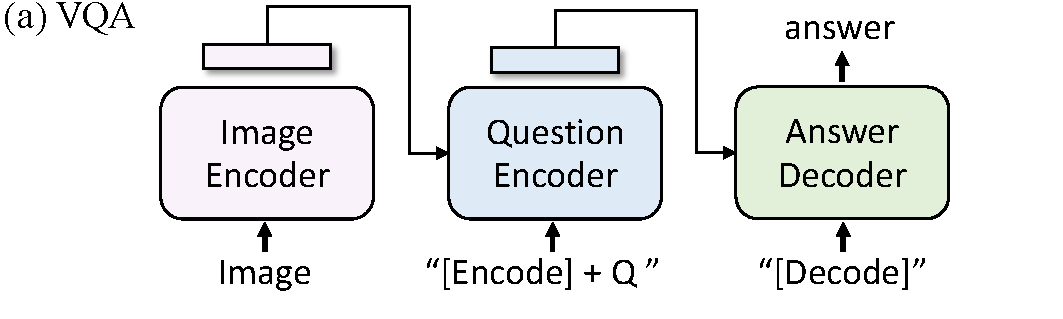
\includegraphics[width=0.98\columnwidth]{imgs/VQA.pdf}
 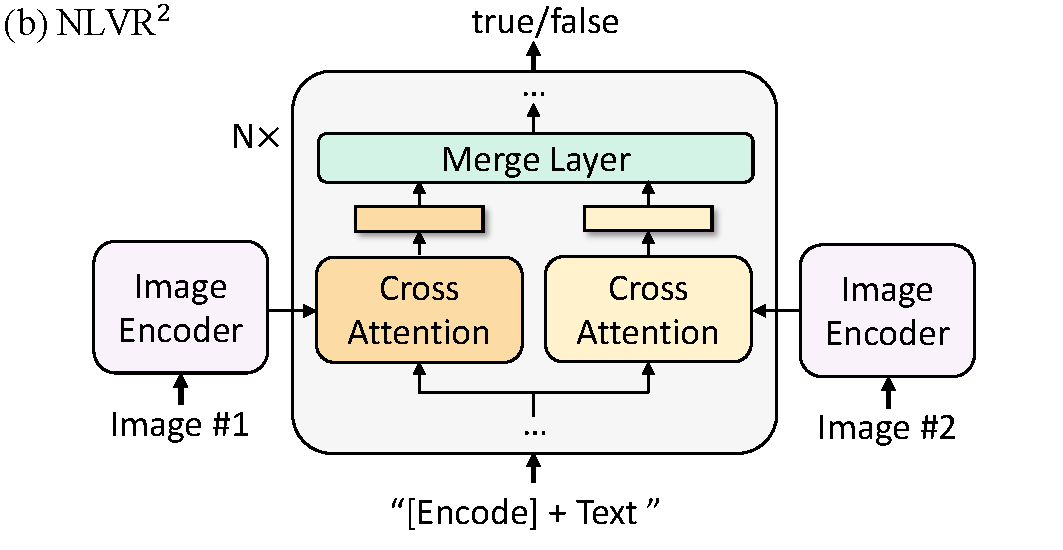
\includegraphics[width=0.98\columnwidth]{imgs/NLVR.pdf}
  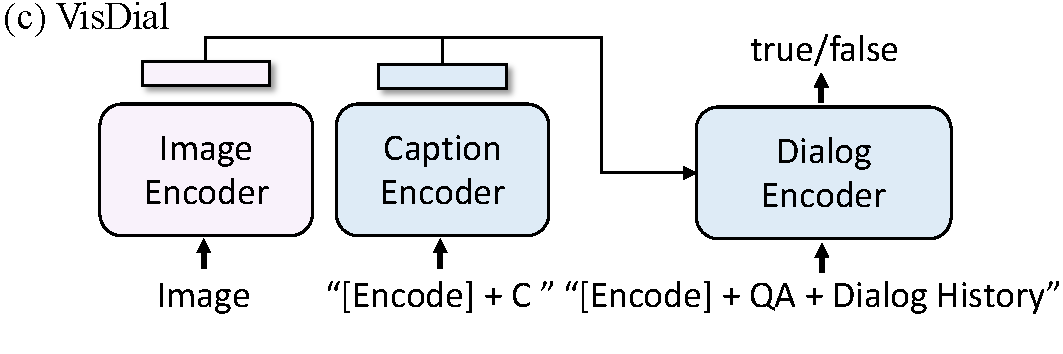
\includegraphics[width=0.98\columnwidth]{imgs/Visdial.pdf}
  \vspace{-3ex}
\caption{Model architecture for the downstream tasks. Q: question; C: caption; QA: question-answer pair.
}
\vspace{-3ex}
\label{fig:vqa_visdial_nlvr}
\end{figure}


\begin{table}[!t]
    % \aboverulesep = 0.48mm
    % \belowrulesep = 0.48mm
    % \small
	\centering	
    \setlength\tabcolsep{5pt}
	\resizebox{1\columnwidth}{!}{%
	\begin{tabular}	{l l  |  c  c  c  c}
		\toprule	 	
	 \multirow{2}{*}{Method}& \multirow{2}{*}{\makecell[l]{Pre-train \\ \#Images}}&  \multicolumn{2}{c}{VQA} & \multicolumn{2}{c}{NLVR$^2$} \\
	  & & test-dev & test-std & dev & test-P \\
	  \midrule
% 	  VisualBERT~\cite{VisualBERT} & 70.80 & 71.00 & 67.40 & 67.00 & - & - \\
% 	  VL-BERT~\cite{VL-BERT} & 71.16 & - &  - & - & - & - \\
	  LXMERT& 180K & 72.42 & 72.54 & 74.90 & 74.50  \\
% 	  12-in-1~\cite{12in1} & 73.15 & - & - & 78.87 & - & 76.95 \\
	  UNITER& 4M & 72.70 & 72.91 & 77.18 & 77.85 \\
	   VL-T5/BART & 180K & - & 71.3 & - & 73.6 \\
	   %ViLT~\cite{ViLT}  & 70.94 & - & 75.24 & 76.21& - & - \\
	   OSCAR& 4M & 73.16 & 73.44 & 78.07 & 78.36 \\
	   SOHO& 219K & 73.25 &73.47 &76.37 &77.32\\
	   VILLA& 4M & 73.59 & 73.67 & 78.39 & 79.30\\
	   UNIMO & 5.6M & 75.06 & 75.27 & - & - \\
	   ALBEF & 14M & 75.84 & 76.04 & \textcolor{lightgray}{82.55} & \textcolor{lightgray}{83.14}\\ 
	   SimVLM$_\mathrm{base}$\dag & 1.8B & 77.87 & 78.14 & 81.72 & 81.77 \\
	   \midrule
	   \name &14M & 77.54 & 77.62 & \textbf{82.67} & 82.30 \\
	   \name & 129M & 78.24 & 78.17 & 82.48 & \textbf{83.08} \\
	   \name$_\text{CapFilt-L}$ & 129M & \textbf{78.25} & \textbf{78.32} & 82.15 & 82.24 \\
	   %\midrule
	   %\midrule
	   %SimVLM$_\mathrm{large}$\dag & 1.8B & 79.32 & 79.56 & 84.13 & 84.84 \\
	   %\name$_\mathrm{large}$  &129M &  &  & 84.07 & 83.47 \\
	\bottomrule
	\end{tabular}
 	}
 \vspace{-2ex}
	\caption
	{
	\small	
		Comparison with state-of-the-art methods on VQA and NLVR$^2$. 
		ALBEF performs an extra pre-training step for NLVR$^2$.
		SimVLM\dag~uses 13$\times$ more training data and a larger vision backbone (ResNet+ViT) than \name.
	}
	\label{tbl:vqa_nlvr}
	\vspace{-4ex}
\end{table}		


VQA~\cite{VQA} requires the model to predict an answer given an image and a question.
Instead of formulating VQA as a multi-answer classification task~\cite{uniter,oscar},
we follow~\citet{ALBEF} and consider it as an answer generation task,
which enables open-ended VQA.
As shown in Figure~\ref{fig:vqa_visdial_nlvr}(a),
during finetuning,
we rearrange the pre-trained model,
where an image-question is first encoded into multimodal embeddings and then given to an answer decoder.
The VQA model is finetuned with the LM loss using ground-truth answers as targets.

The results are shown in Table~\ref{tbl:vqa_nlvr}.
Using 14M images, \name~outperforms ALBEF by +1.64\% on the test set.
Using 129M images, \name~achieves better performance than SimVLM which uses $13\times$ more pre-training data and a larger vision backbone with an additional convolution stage.

\vspace{-1ex}
\subsection{Natural Language Visual Reasoning (NLVR$^2$)}
\vspace{-0.5ex}
NLVR$^2$~\cite{NLVR} asks the model to predict whether a sentence describes a pair of images.
In order to enable reasoning over two images,
we make a simple modification to our pre-trained model which leads to a more computational-efficient architecture than previous approaches~\cite{ALBEF,simvlm}.
As shown in Figure~\ref{fig:vqa_visdial_nlvr}(b),
for each transformer block in the image-grounded text encoder,
there exist two cross-attention layers to process the two input images,
and their outputs are merged and fed to the FFN.
The two CA layers are intialized from the same pre-trained weights.
The merge layer performs simple average pooling in the first 6 layers of the encoder,
and performs concatenation followed by a linear projection in layer 6-12.
An MLP classifier is applied on the output embedding of the \texttt{[Encode]} token.
As shown in Table~\ref{tbl:vqa_nlvr},
\name~outperforms all existing methods except for ALBEF which performs an extra step of customized pre-training.
Interestingly,
performance on NLVR$^2$ does not benefit much from additional web images,
possibly due to the domain gap between web data and downstream data.



\vspace{-1ex}
\subsection{Visual Dialog (VisDial)}
\vspace{-0.5ex}
VisDial~\cite{VisDial} extends VQA in a natural conversational setting,
where the model needs to predict an answer not only based on the image-question pair, but also considering the dialog history and the image's caption.
We follow the discriminative setting where the model ranks a pool of answer candidates~\cite{ReDAN,VD-BERT,visdial_eccv}.
As shown in Figure~\ref{fig:vqa_visdial_nlvr}(c),
we concatenate image and caption embeddings,
and pass them to the dialog encoder through cross-attention.
The dialog encoder is trained with the ITM loss to discriminate whether the answer is true or false for a question,
given the entire dialog history and the image-caption embeddings.
As shown in Table~\ref{tbl:visdial},
our method achieves state-of-the-art performance on VisDial v1.0 validation set.
% We also perform zero-shot experiments where we directly evaluate the open-ended VQA model without dialog history.

\vspace{-1ex}
\subsection{Zero-shot Transfer to Video-Language Tasks}
\vspace{-0.5ex}

\begin{table}[!t]
    % \aboverulesep = 0.48mm
    % \belowrulesep = 0.48mm
    \small
	\centering	
    \setlength\tabcolsep{5pt}
	\resizebox{1\columnwidth}{!}{%
	\begin{tabular}	{l   |  c  c  c  c c }
		\toprule	 	
	 Method & MRR$\uparrow$ & R@1$\uparrow$ & R@5$\uparrow$ & R@10$\uparrow$ & MR$\downarrow$  \\
		\midrule
% 		\multicolumn{6}{l}{\textit{finetuning}}\\
% 		\midrule
	   % ReDAN &  53.13 & 41.38 & 66.07 & 74.50 & 8.91 \\
        VD-BERT & 67.44 & 54.02 & 83.96 & 92.33 & 3.53 \\
        VD-ViLBERT\dag & 69.10 & 55.88 & 85.50 & 93.29 & 3.25\\
        \name & \textbf{69.41} & \textbf{56.44} & \textbf{85.90} & \textbf{93.30}& \textbf{3.20}\\
% 		\midrule
% 		\multicolumn{6}{l}{\textit{zero-shot}}\\
% 		\midrule     
% 		VD-ViLBERT & 6.88 & 2.63 & 7.17 & 11.30 & 46.90 \\ \name-VQA & & & & & \\
		\bottomrule
	\end{tabular}
 	}
 \vspace{-2ex}
	\caption
	{
	\small	
		Comparison with state-of-the-art methods on VisDial v1.0 validation set. VD-ViLBERT\dag~\cite{visdial_eccv} pre-trains ViLBERT~\cite{ViLBERT} with additional VQA data.
	}
	\vspace{-3ex}
	\label{tbl:visdial}
\end{table}		
\begin{table}[!t]

 \resizebox{1\columnwidth}{!}{
    % \aboverulesep = 0.55mm
    % \belowrulesep = 0.55mm
 	% \small
	\centering	
      \setlength\tabcolsep{4pt}
		\begin{tabular}	{l  |  c c c c}
		\toprule
		Method & R1$\uparrow$ & R5$\uparrow$ & R10$\uparrow$ & MdR$\downarrow$\\
		\midrule
		\multicolumn{3}{l}{\textit{zero-shot}}\\
		\midrule
% 		HT100M~\cite{miech2019howto100m} & 7.5 & 21.2 & 29.6 & 38\\ 
		ActBERT~\cite{zhu2020actbert} & 8.6 & 23.4 & 33.1 & 36\\
		SupportSet~\cite{patrick2021supportset} & 8.7 & 23.0 & 31.1 & 31\\
        MIL-NCE~\cite{miech2020end} & 9.9 & 24.0 & 32.4 & 29.5\\ VideoCLIP~\cite{xu2021videoclip} & 10.4 & 22.2 & 30.0 & -\\
        FiT~\cite{FiT} & 18.7 & 39.5 & 51.6 & 10 \\ 
        \name & \textbf{43.3} & \textbf{65.6} & \textbf{74.7} & \textbf{2} \\
        \midrule
        \multicolumn{3}{l}{\textit{finetuning}}\\
        \midrule
        ClipBERT~\cite{lei2021less} & 22.0 & 46.8 & 59.9 & 6 \\
        VideoCLIP~\cite{xu2021videoclip} & 30.9 & 55.4  & 66.8 & - \\
        \bottomrule
		\end{tabular}
 		}
 	\vspace{-2ex}
    \caption
	{Comparisons with state-of-the-art methods for text-to-\textbf{video} retrieval on the 1k test split of the MSRVTT dataset.}
	\vspace{-1ex}
	\label{tbl:video_retrieval}
\end{table}		
\begin{table}[!t]

 \resizebox{1\columnwidth}{!}{
    % \aboverulesep = 0.55mm
    % \belowrulesep = 0.55mm
 	% \small
	\centering	
     \setlength\tabcolsep{5pt}
		\begin{tabular}	{l  |  c c }
		\toprule
		Method & MSRVTT-QA& MSVD-QA\\
		\midrule
		\multicolumn{3}{l}{\textit{zero-shot}}\\
		\midrule		
		VQA-T~\cite{justask} &  2.9 & 7.5 \\
		\name & 19.2 & 35.2 \\ 
		\midrule
		\multicolumn{3}{l}{\textit{finetuning}}\\
		\midrule
		HME~\cite{fan2019heterogeneous}  & 33.0 & 33.7 \\
    	HCRN~\cite{le2020hierarchical}  & 35.6 & 36.1 \\
% 		ClipBERT~\cite{lei2021less} & 37.4 & - \\
% 		SSML~\cite{amrani2021noise}  & 35.1 & 35.1 \\
% 		CoMVT~\cite{comvt}  & 39.5 & 42.6 \\
		VQA-T~\cite{justask} & 41.5 & 46.3\\		
        \bottomrule
		\end{tabular}
		}
    \vspace{-2ex}		
    \caption
	{Comparisons with state-of-the-art methods for  \textbf{video} question answering. We report top-1 test accuracy on two datasets.}
	\vspace{-3ex}
	\label{tbl:video_qa}
\end{table}		


Our image-language model has strong generalization ability to video-language tasks.
In Table~\ref{tbl:video_retrieval} and Table~\ref{tbl:video_qa},
we perform zero-shot transfer to \textit{text-to-video retrieval} and \textit{video question answering},
where we directly evaluate the models trained on COCO-retrieval and VQA, respectively.
To process video input,
we uniformly sample $n$ frames per video ($n=8$ for retrieval and $n=16$ for QA),
and concatenate the frame features into a single sequence.
Note that this simple approach ignores all temporal information.

Despite the domain difference and lack of temporal modeling,
our models achieve state-of-the-art performance on both video-language tasks.
For text-to-video retrieval,
zero-shot \name~even outperforms models finetuned on the target video dataset by +12.4\% in recall@1.
Further performance improvement can be achieved if the \name~model is used to initialize a video-language model with temporal modeling (\eg~replace our ViT with a TimeSformer~\cite{timesformer}) and finetuned on video data.



